The Odin middleware is designed to be adaptable and extensible, adopting procedures that are readily available in most relational database systems. The current prototype is built on top of PostgreSQL to enhance its optimization capabilities without replacing or discarding its optimizer completely. This section goes through the actual implementation details of each module.

\subsection{Parser and Featurizer}

This module has the task of parsing \gls{sql} statements and generate a vector representation of each alternative execution plan.

\subsubsection{Parser}

The parser reads \gls{sql} statements and interacts with the underlying \gls{dbms} interface to get an idea of how the optimizer intends to execute the query without actually running it. Most database systems come with a built-in explainer that tells how the query planner will execute a particular SQL query (e.g., \textit{EXPLAIN} command in the case of PostgreSQL). As shown in Figure \ref{fig:explain_command}, it allows targeting query performance specifics such as: (1) how the tables referenced by the statement will be scanned, (2) if multiple tables are referenced, information about what join algorithms will be used to bring together the required rows from each input table and (3) cardinality estimates and predicted execution time.

\begin{figure}[H]
\centering
\begin{minipage}{0.72\textwidth}
\begin{minted}[frame=lines,
               framesep=2mm,
               fontsize=\small,
               mathescape=true,
               escapeinside=||
]{Text}
EXPLAIN SELECT * FROM foo;

                       QUERY PLAN
---------------------------------------------------------
 Seq Scan on foo  (cost=0.00..155.00 rows=10000 width=4)
(1 row)
\end{minted}
\end{minipage}
\caption{Example of the output of an \textit{EXPLAIN} command output}
\label{fig:explain_command}
\end{figure}

\subsubsection{Featurizer}

The featurizer takes the execution plan that the PostgreSQL planner generates for the supplied statement and converts it to a vector of fixed dimensions for machine learning algorithms to interpret it. It provides a simple interface of two methods representing execution plans at two different granularities to support two different types of machine learning algorithms.

\paragraph{Plan-level Featurization}

In this method, the query plan is represented as a single vector and ignores lower-level details, such as the position and order between different operators. Instead, as illustrated in Figure \ref{fig:plan_level_featurization}, it uses a set of features containing estimates, such as operator cardinalities and execution times, together with the occurrence count of each operator type in the query plan.

\begin{figure}[H]
\centering
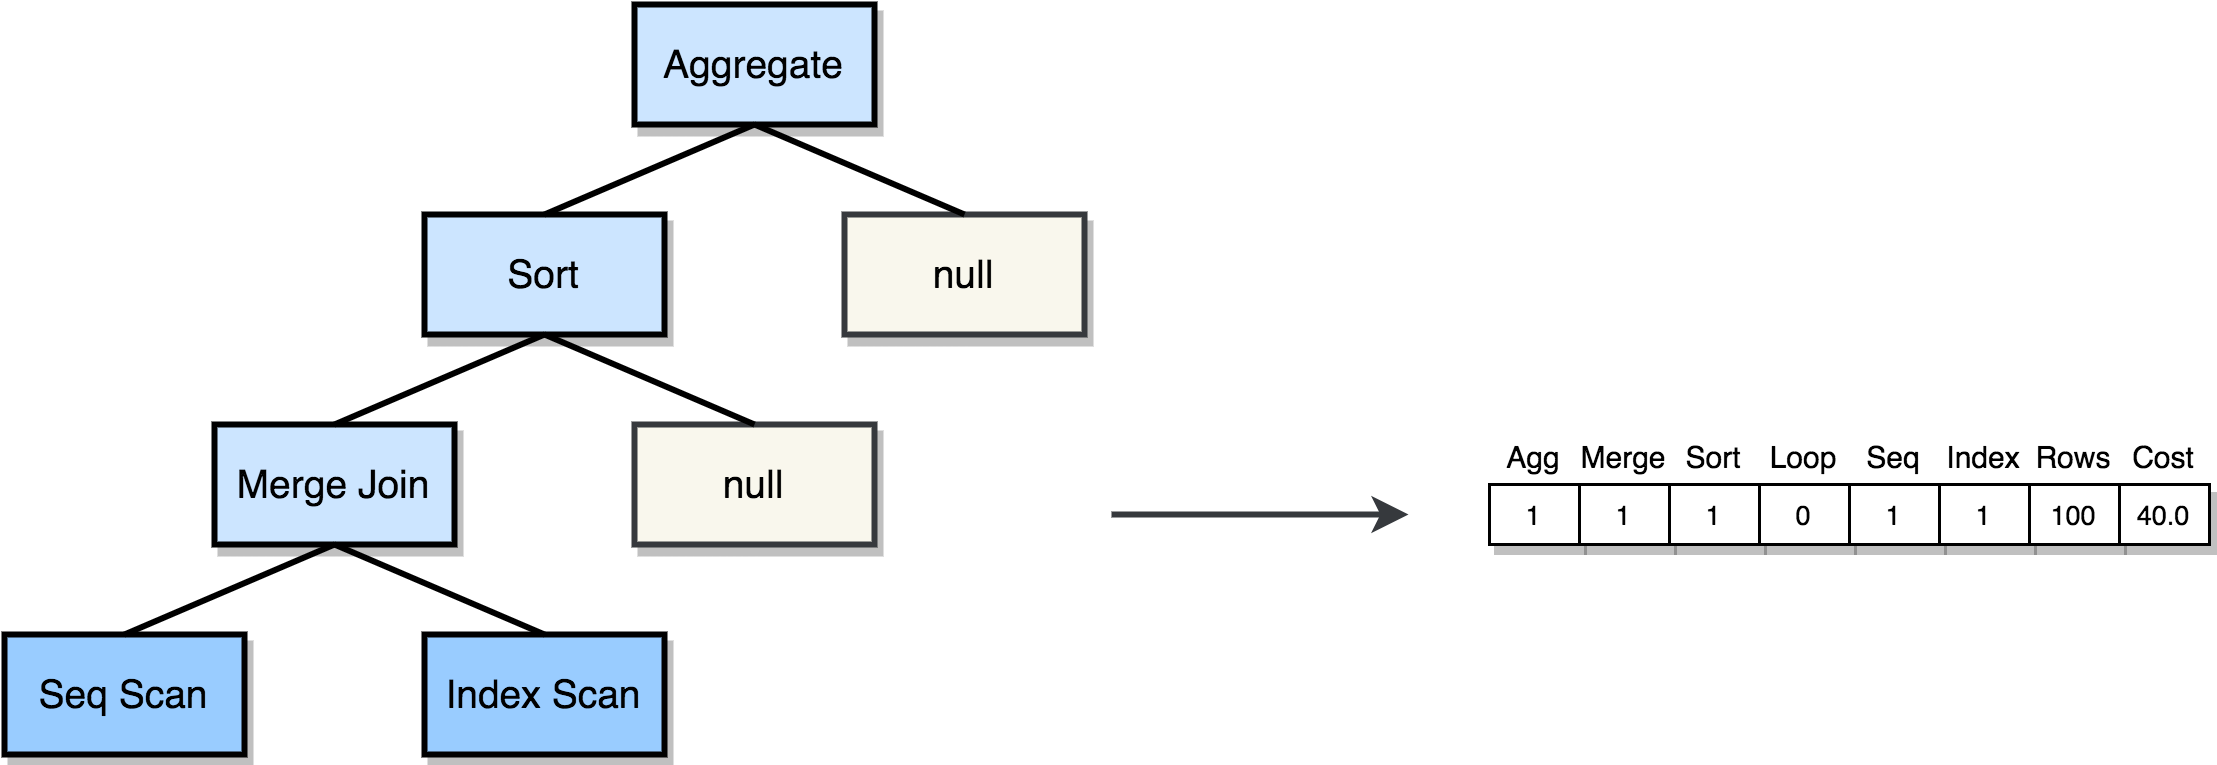
\includegraphics[width=0.9\textwidth]{img/solution/plan_level_featurization.png}
\caption{Plan-level featurization}
\label{fig:plan_level_featurization}
\end{figure}

This approach was devised to be used directly in more traditional machine learning approaches. Additionally, it is model agnostic and can readily work with different model types.

\paragraph{Operator-level Featurization}

This method encodes a query plan as a tree of vectors and preserves its inherent tree structure by binarizing the query plan tree and encoding each operator as a vector. As shown in Figure \ref{fig:operator_level_featurization}, each node is annotated by the physical operator being used and some optimizer estimates, such as estimated operator cost and cardinality. The process of binarization includes transforming non-binary query plans into binary ones by introducing \textit{null} nodes. Therefore, each tree node has exactly two or zero children. 

\begin{figure}[H]
\centering
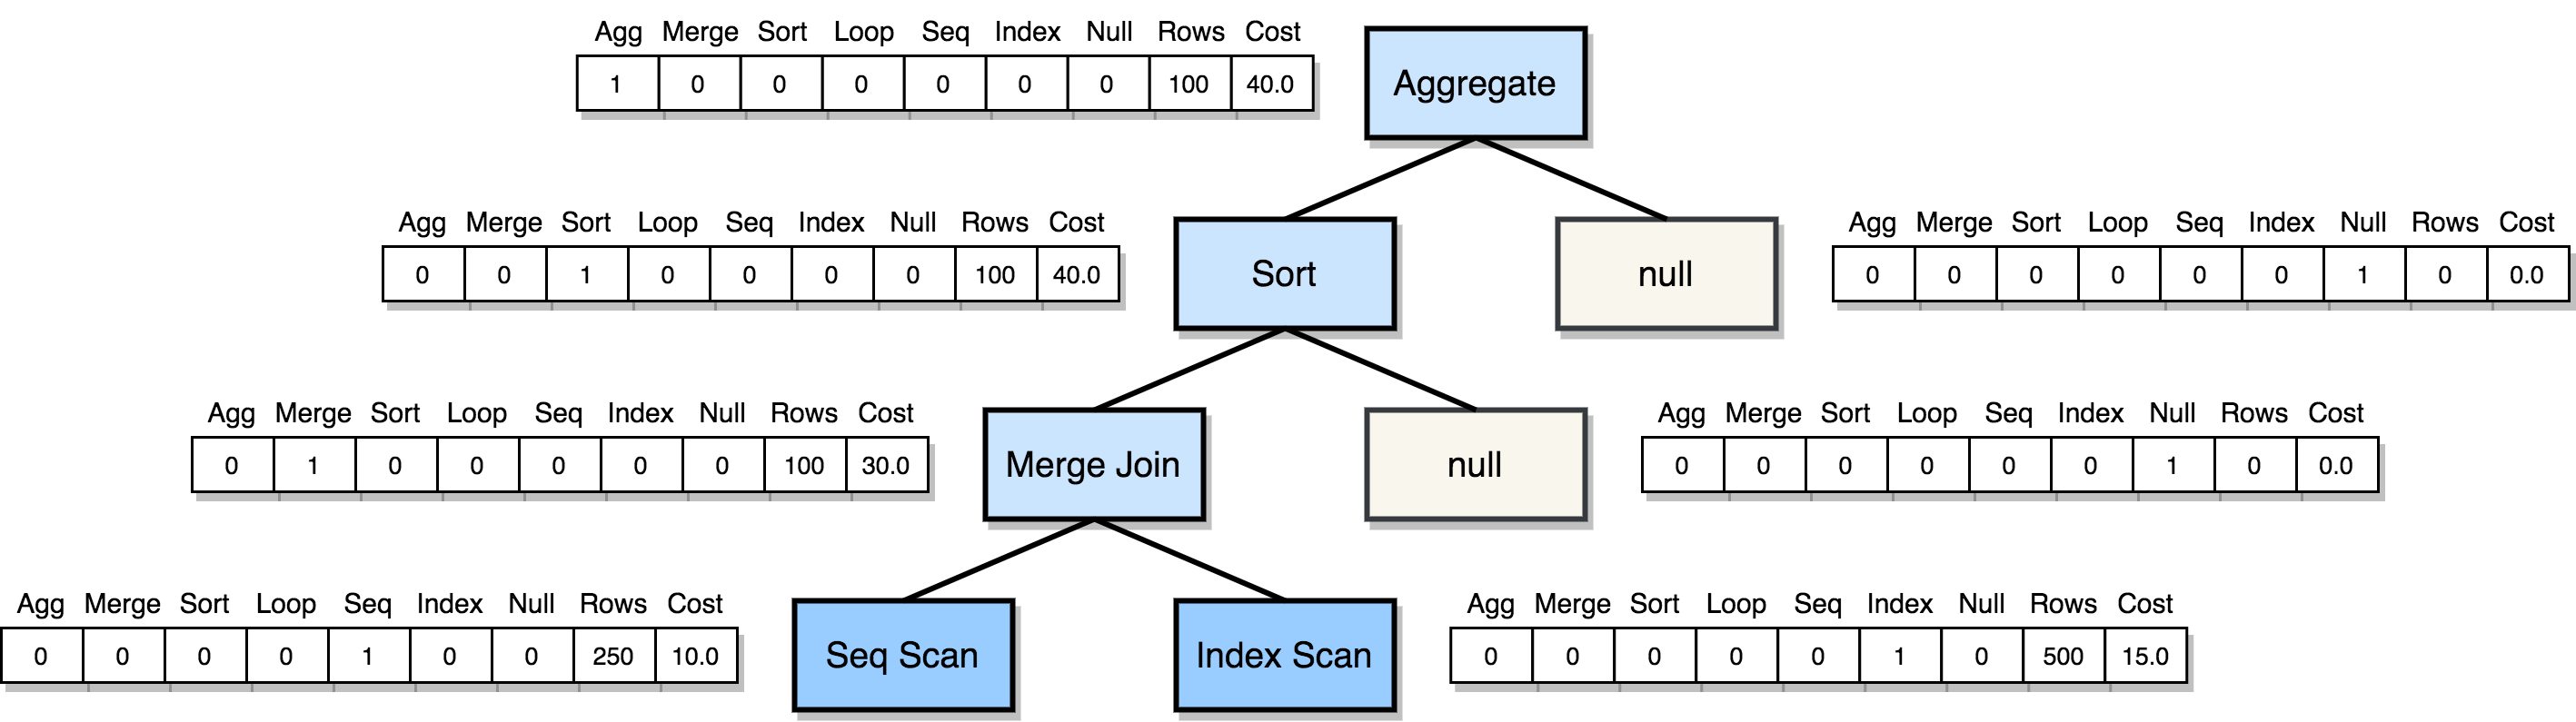
\includegraphics[width=\textwidth]{img/solution/operator_level_featurization.png}
\caption{Operator-level featurization}
\label{fig:operator_level_featurization}
\end{figure}

This featurization approach was first designed in Bao \citep{Marcus2020} and was implemented in Odin to feed the deep learning algorithm described in the following section.

\subsection{Learning Module}

The learning module was devised to have a central role within the system and is responsible for loading pre-trained predictive models to infer the cost of an execution plan having its vector representation as input and building and storing new ones.

The main focal point of Odin is comparing the execution cost of two plans of the same query corresponding to different optimizer configurations. Instead of relying on the optimizer's estimates and cost model for such comparison, Odin models the cost estimation of executing a plan as a regression task as follows:

\begin{quote}
Given a query plan $P$ for a query $Q$ chosen by the optimizer under configuration $C$, the goal is to predict the cost of executing $P$ in terms of execution time.    
\end{quote}

\subsubsection{Predictive Models}

When it comes to predictive models, both traditional algorithms and deep learning approaches should be considered. Using deep neural networks is a computationally heavy task that requires a considerable amount of useful and labeled data. For this reason, more often than not, it might be an overkill approach for more straightforward problems. One simpler approach is to use traditional algorithms, such as linear or tree models to train the predictive model. To make Odin extensible, it supports both types of models allowing to observe whether the use of deep learning is justified.

\paragraph{Traditional Algorithms} 

Odin employs several types of traditional algorithms such as linear regression, a regression variant of Support Vector Machines (\gls{svms}), and Random Forests (\gls{rf}) models for predicting the execution cost of a given plan.

\begin{figure}[ht]
\centering
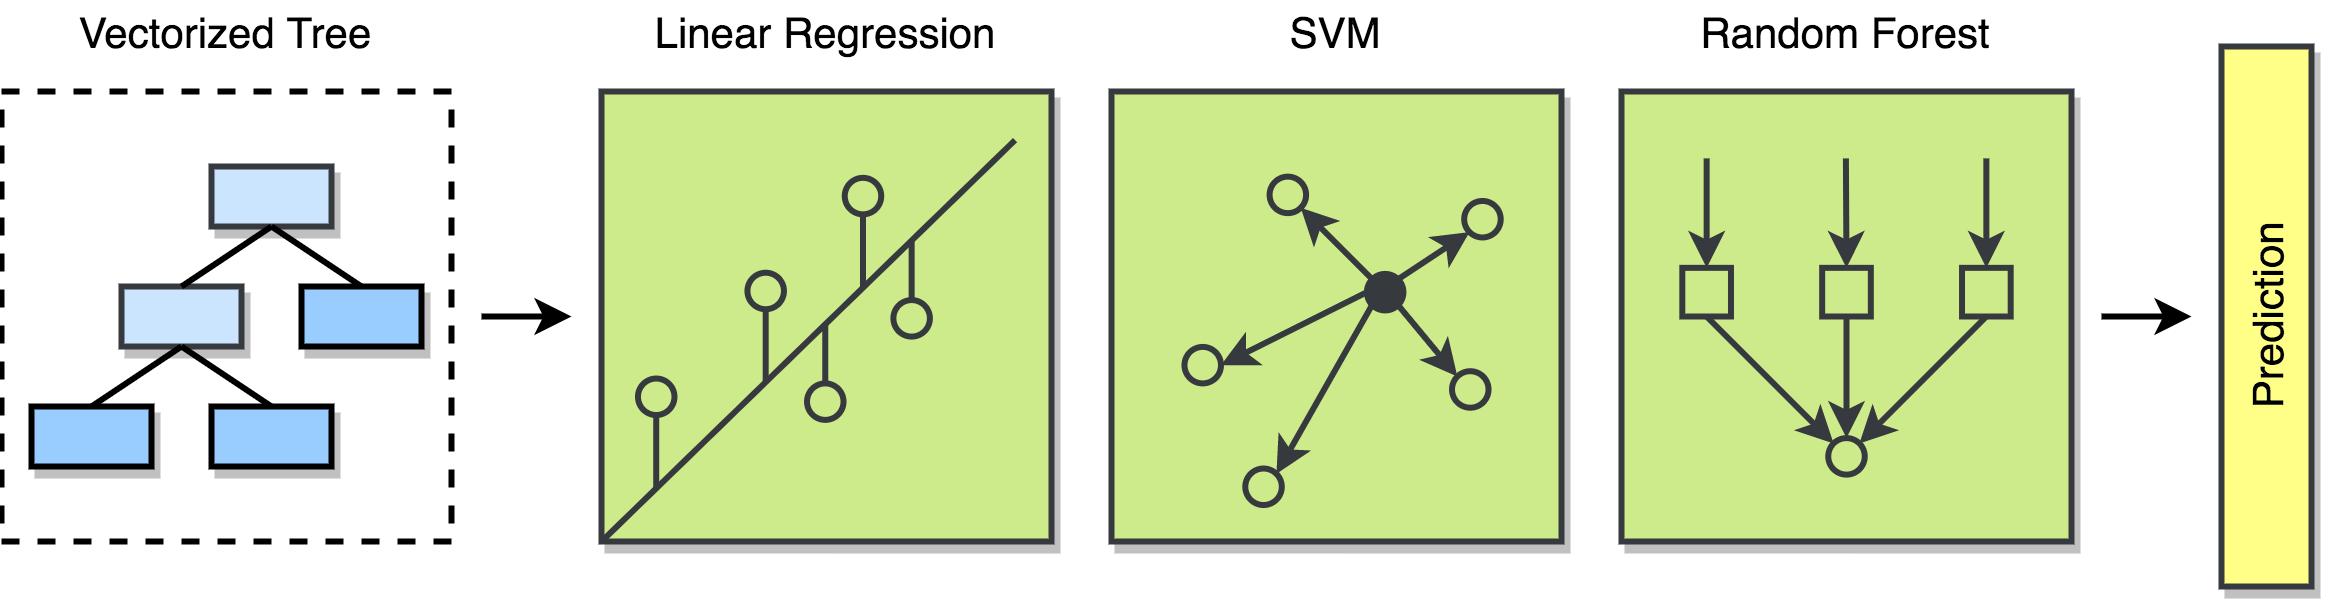
\includegraphics[width=\textwidth]{img/solution/traditional_algorithms.png}
\caption{Traditional machine learning algorithms}
\label{fig:traditional_algorithms}
\end{figure}

As shown in Figure \ref{fig:traditional_algorithms}, for these traditional algorithms, each query plan is featurized into a single vector using the plan-level featurization strategy described earlier.

\paragraph{Tree Convolutional Neural Network} 

A tree convolutional neural network (\gls{tcnn}) is a specialized type of \gls{cnn} that was adapted effectively to query plan trees, providing the ability to automatically learn a large number of filters on a given training data set for query execution time prediction \citep{Marcus2020}.

As in conventional convolutional neural networks, a convolution layer applies several filters to an input tree. The systematic application of the same filter across a query plan allows discovering patterns in the input data. For instance, these filters may look for patterns like pairs of hash joins or an index scan over a small relation.

\begin{figure}[ht]
\centering
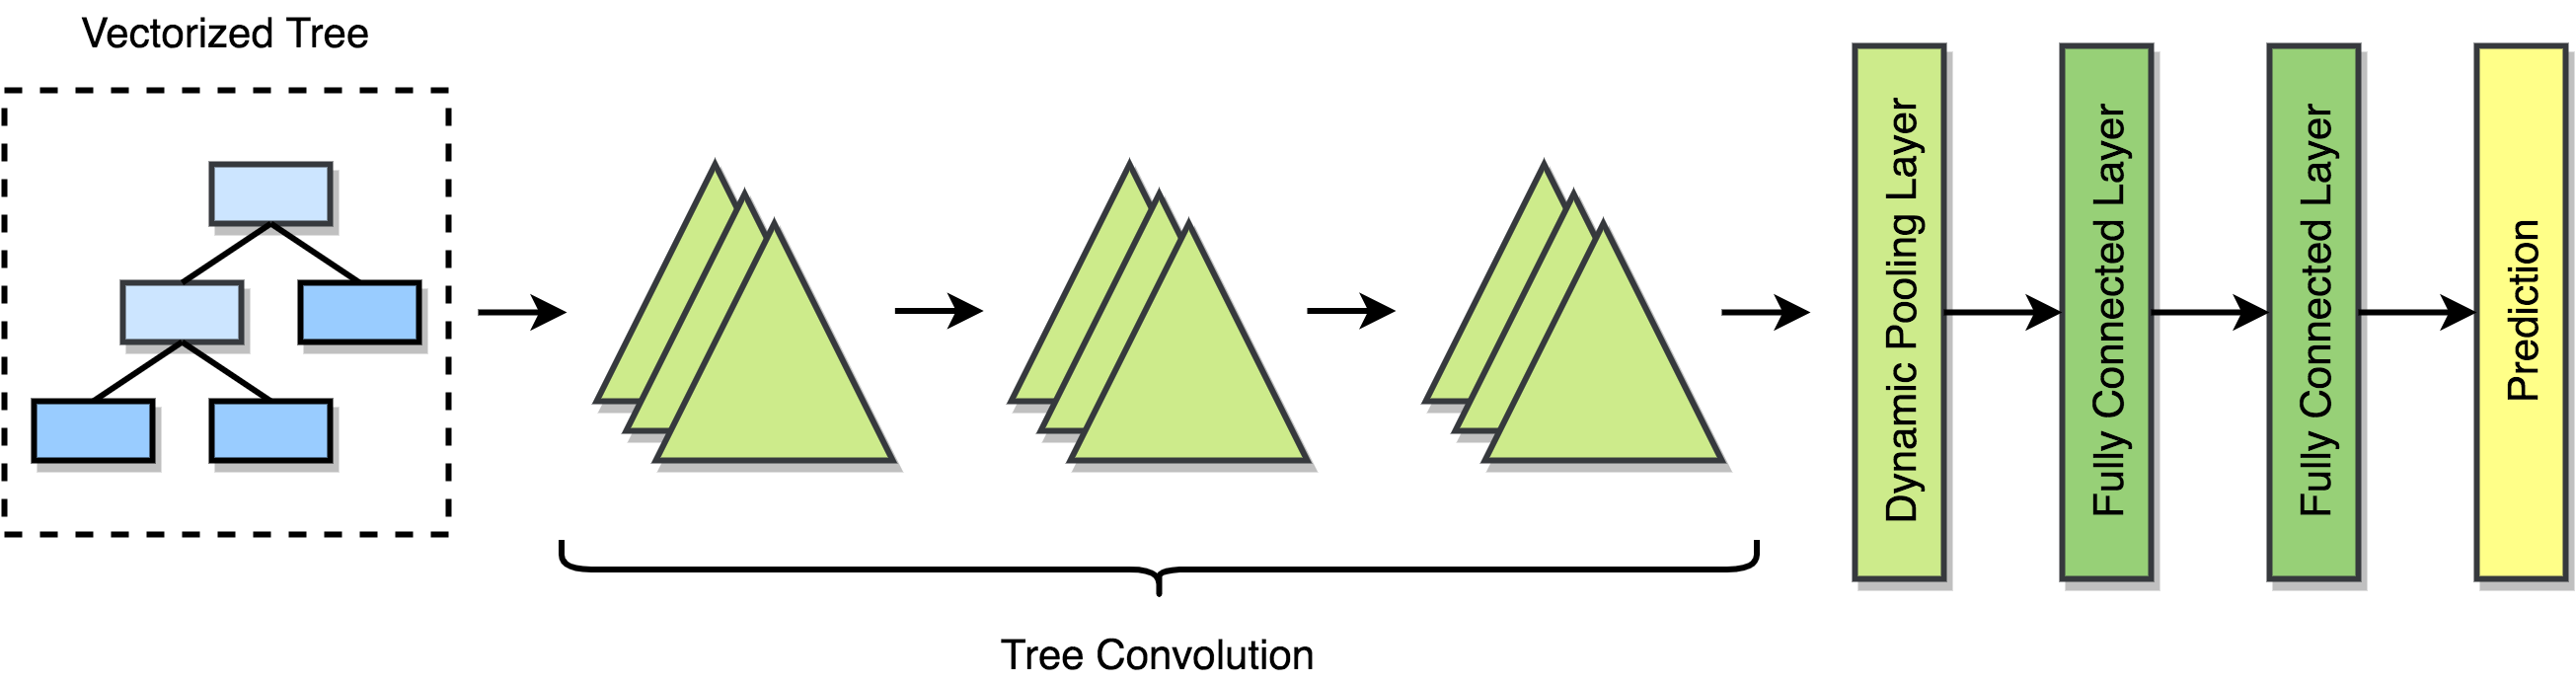
\includegraphics[width=\textwidth]{img/solution/tree_convolutional_neural_network.png}
\caption{Tree convolutional neural network}
\label{fig:tree_convolutional_neural_network}
\end{figure}

Figure \ref{fig:tree_convolutional_neural_network} shows the overall architecture of a \gls{tcnn}. As the output of a tree convolution is another tree, multiple layers of tree convolution filters can be stacked. While the first convolution layer learns simple features (e.g., recognizing a merge join on top of a merge join), the last tree convolution layer learns complex features (e.g., recognizing a left-deep chain of merge joins).

After the query plan tree is passed through a set of tree-based convolutional kernels to extract a query plan's structural information, Odin applies dynamic pooling to gather information over different parts of the tree. Then, a hidden layer and an output layer are added. Finally, two fully connected layers are used to map the pooled vector to predict the execution cost of the given plan.

\subsection{Configuration Tuner}

The configuration tuner is the main module within the system. It has the task of interacting with the PostgreSQL client interface and learning to select the set of strategies that result in the lowest runtime for a particular query. Concerning the actual implementation, this module has two main functions:

\begin{itemize}
    \item Predictive model training: The tuner interacts with the learning module to generate predictive models from a set of \gls{sql} queries that the user specifies as input;
    \item Optimizer configuration tuning: The tuner uses one of the previously generated predictive models to evaluate the best set of strategies for a particular query served as input, returning the result of its execution.
\end{itemize}

\subsubsection{Predictive Model Training}

Besides loading pre-trained predictive models to infer the cost of an execution plan, the configuration tuner module also allows generating and storing new ones. Considering the use of a supervised machine learning approach, Odin relies on historical data to train one of the supported models. Thus, the model training process is based on two basic assumptions:

\begin{itemize}
    \item There is a sample workload (i.e., a set of \gls{sql} queries) representative of the user's total workload;
    \item A traditional query optimizer, such as PostgreSQL, should be used to create valid query execution plans for each query in the sample workload.
\end{itemize}

\begin{figure}[H]
\centering
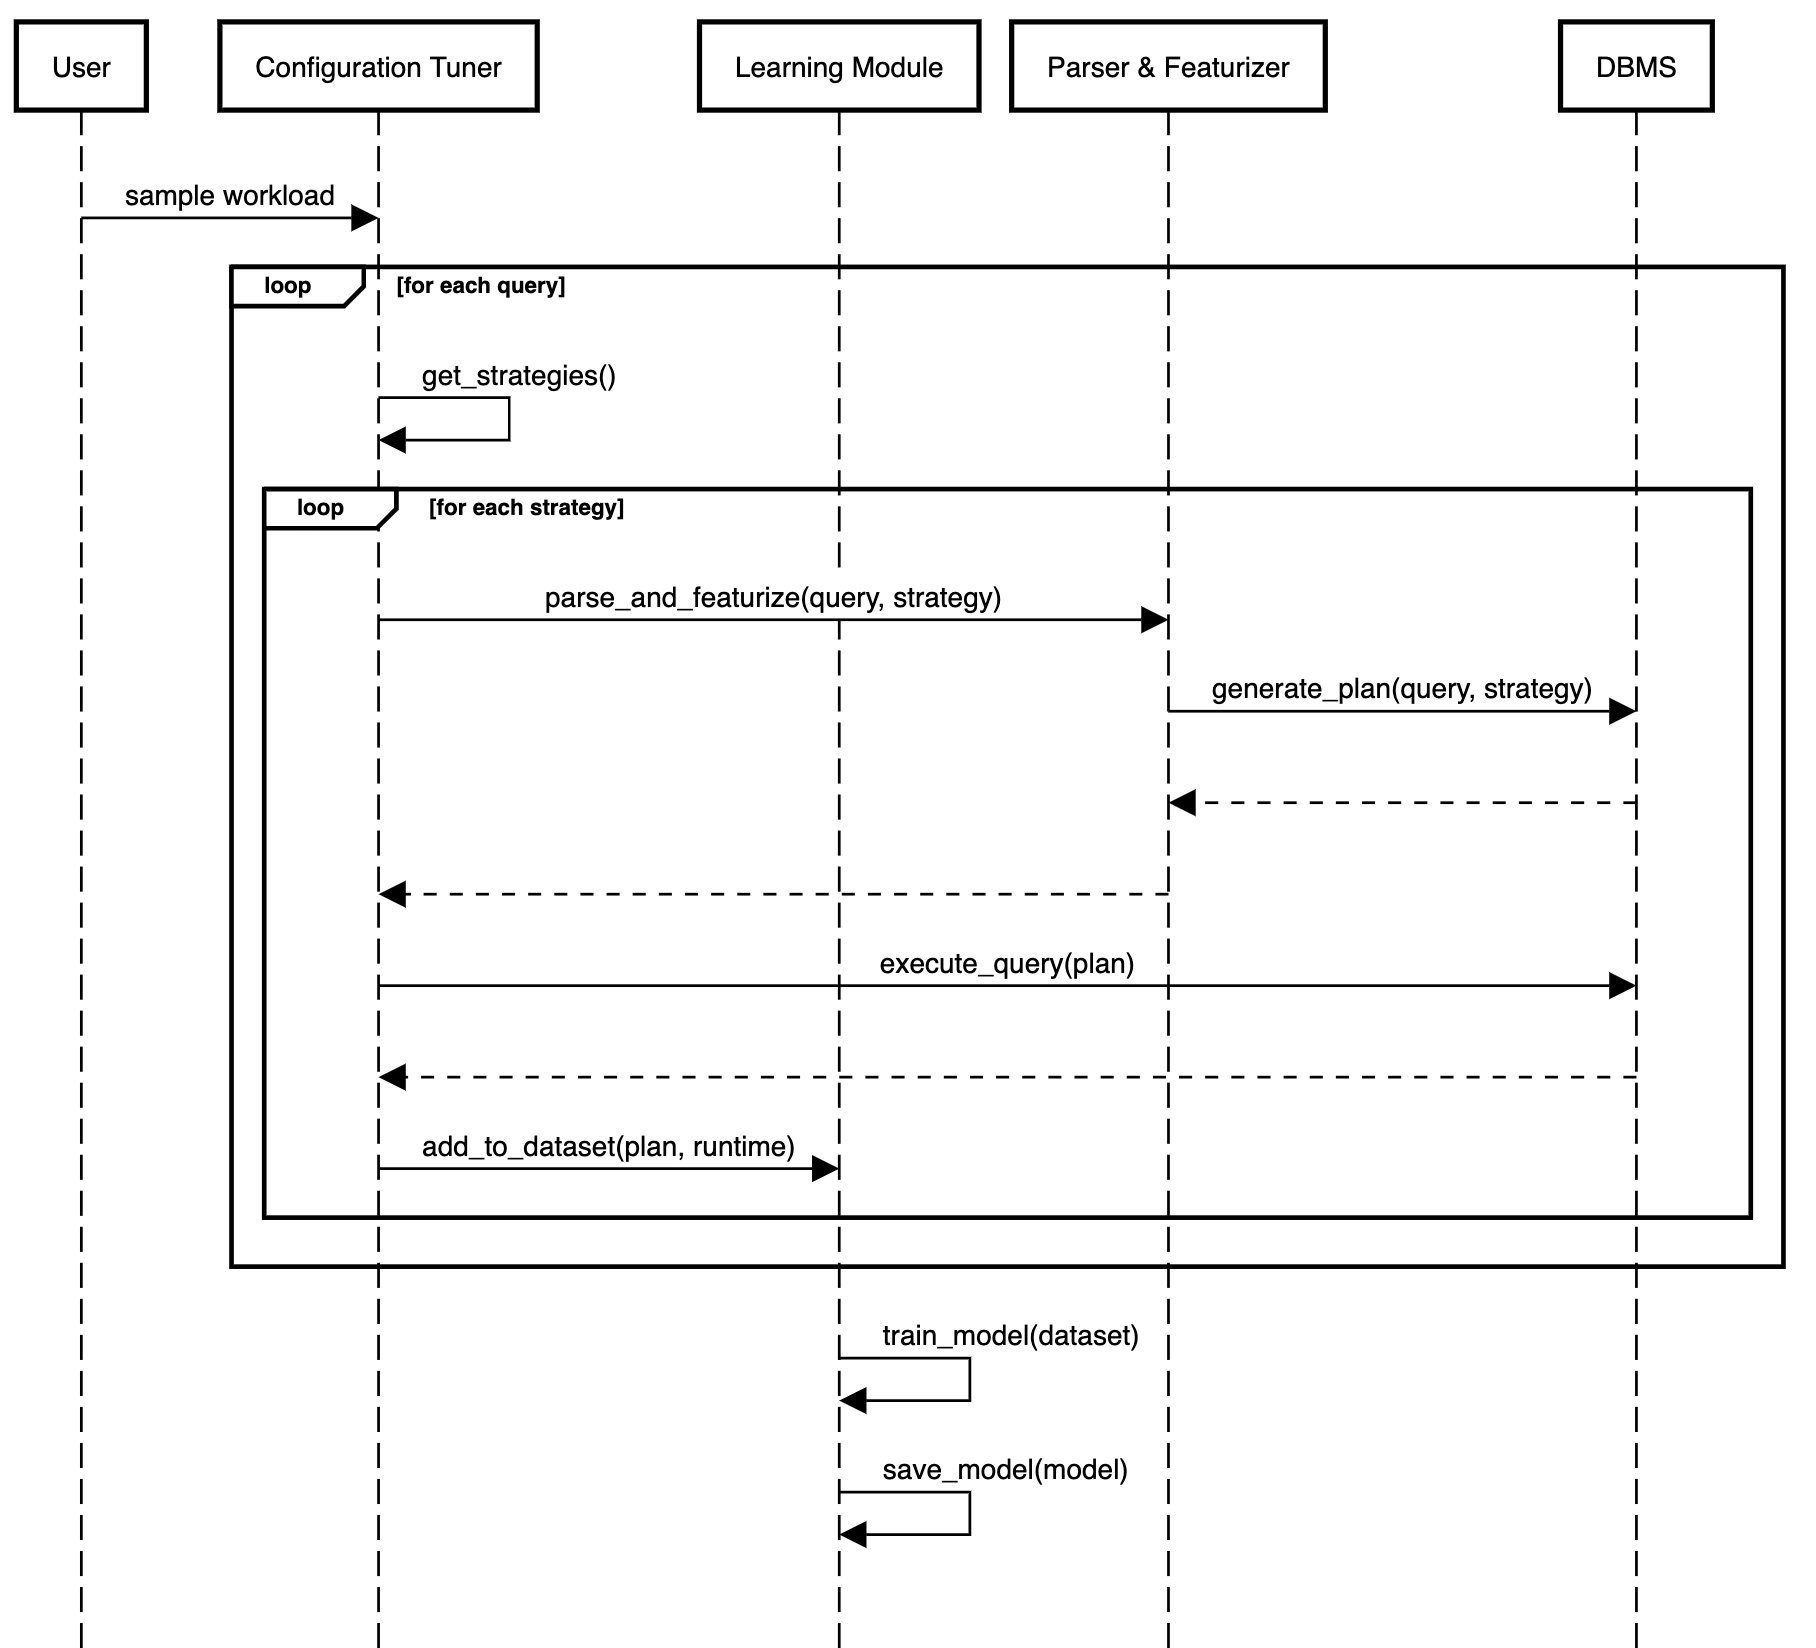
\includegraphics[width=\textwidth]{img/solution/training_sequence_diagram.png}
\caption{Odin's predictive model training}
\label{fig:training_sequence_diagram}
\end{figure}

Figure \ref{fig:training_sequence_diagram} illustrates how this module generates predictive models with the specified sample workload. First, for each query of the sample workload, the configuration tuner generates several plans under different strategy settings. Then, it interacts with the parser and featurizer module to obtain a vectorized representation of the query plan. Finally, it interacts with PostgreSQL to execute each plan and build a model relying on a data set with the plans vectorized representations and their corresponding execution times.

\subsubsection{Configuration Analysis and Selection}

This section discusses the approach to configuration analysis and selection. The problem can be formulated as follows:

\begin{quote}
Given a query $Q$, the goal is to find the set of strategy settings, or configuration $C$, that results in the lowest execution $cost(Q, C)$, where $cost(Q, C)$ is the cost of query $Q$ under configuration $C$.
\end{quote}

\begin{figure}[H]
\centering
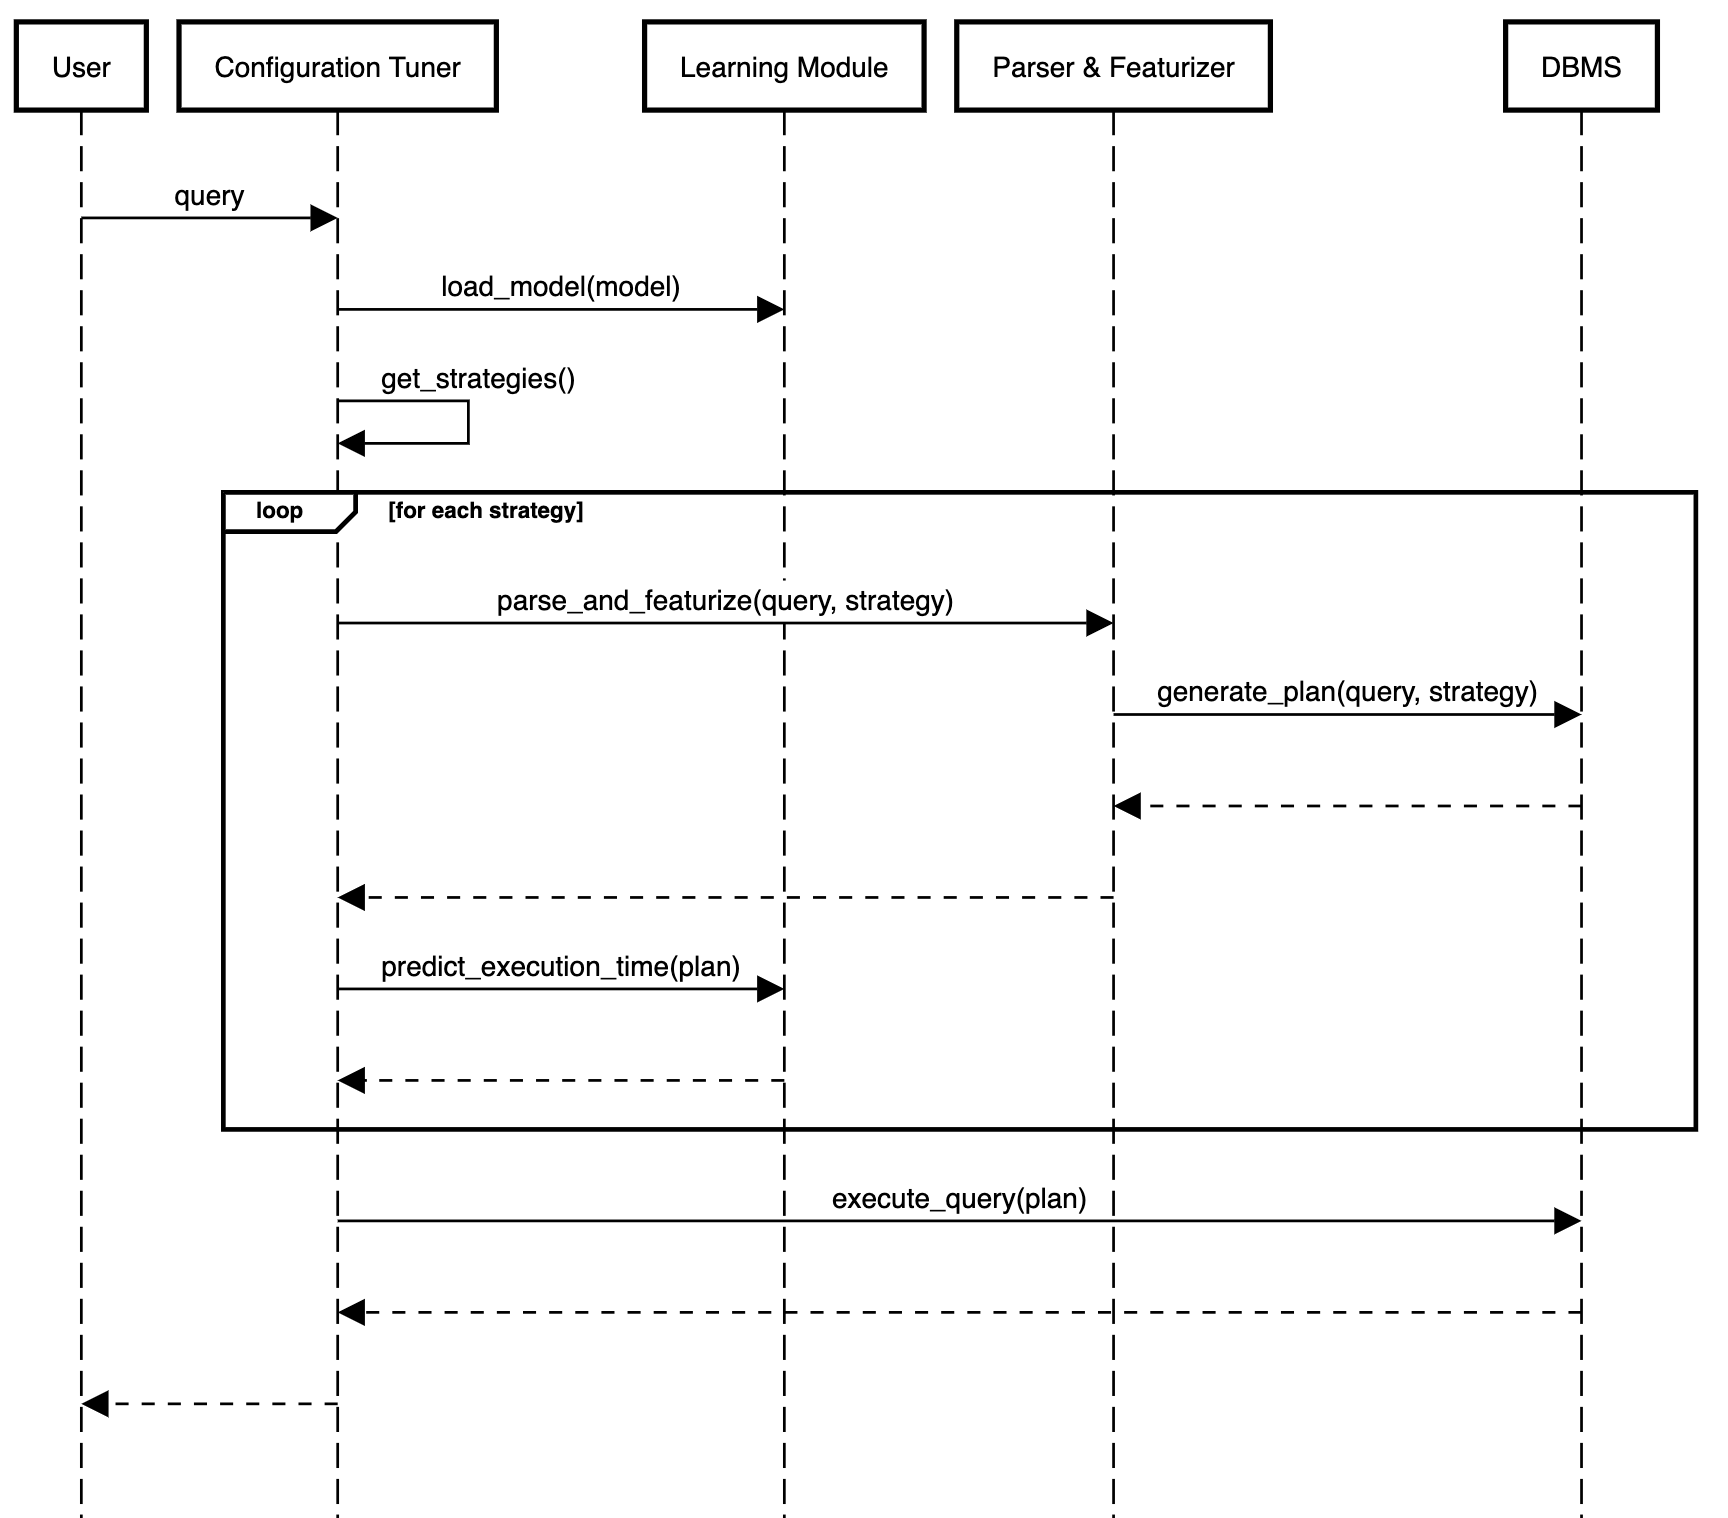
\includegraphics[width=\textwidth]{img/solution/configuration_selection_sequence_diagram.png}
\caption{Odin's configuration analysis and selection}
\label{fig:configuration_analysis_and_selection}
\end{figure}

Figure \ref{fig:configuration_analysis_and_selection} illustrates the steps involved in the process. The configuration tuner starts by interacting with the learning module to load the intended predictive model. Then, it evaluates the effects of disabling certain strategies by interacting with the PostgreSQL client interface to generate query plans under such circumstances. Furthermore, using the cost prediction as its primary input, the configuration tuner sets the configuration with the lowest predicted execution cost following a greedy enumeration algorithm, which is described in further detail in the following section. Finally, it returns the query result to the user.

\paragraph{Plan Enumeration Algorithm}

This section describes how the configuration tuner finds the best configuration for a single query in further detail.

Finding the optimal set of strategy settings requires exhaustive search, which is prohibitively expensive. For this reason, similarly to  index tuners such as \citep{chaudhuri1997}, the plan enumeration algorithm the configuration tuner uses is defined greedily, as illustrated in Figure \ref{fig:greedy_enumeration}. To begin with, a configuration of size $m$ (an arbitrary number where $m \leq k$) must be chosen as a starting point. Then, the algorithm iteratively suggests the rest of the configuration until all $k$ possible strategy settings have been chosen, or no further reduction in execution cost is possible. Each iteration considers all possible choices and adds the one that results in the highest cost reduction.

Since the algorithm requires an arbitrary number \textit{m} as a starting point, it is crucial to find the right balance between the two extremes. On the one hand, if \textit{m = 0}, the algorithm takes a pure greedy approach. On the other hand, if \textit{m = k}, the algorithm is identical to the naive enumeration algorithm. Therefore, the value of \textit{m} relative to \textit{k} reflects the desired degree of completeness of enumeration and is configurable by the user.

\begin{figure}[ht]
\begin{algorithm}[H]
\SetAlgoLined
\DontPrintSemicolon
Let $S$ = the best $m$ configuration using the \textit{naive enumeration algorithm}\\
\Begin{
    1. \textbf{if} $m = k$ \textbf{then} exit\;
    2. Choose a new operator $O$ such that $cost(S \cup \{O\}) \leq cost(S)$ for any choice of\; \hspace{0.3cm} $O \not\in S$\;
    3. \textbf{if} $cost(S \cup \{O_i\}) \geq cost(S)$ \textbf{then exit}\;
      \hspace{0.4cm}{\textbf{else} $S = S \cup \{O_i\}$\;}
    4. \textbf{if} $|S|$ = k \textbf{then exit}\;
    5. \textbf{goto 2}\;
}
$output \longleftarrow$ configuration with minimum cost\;
\caption{Greedy (m, k) enumeration algorithm}
\end{algorithm}
\caption{Odin's greedy enumeration algorithm}
\label{fig:greedy_enumeration}
\end{figure}

\paragraph{Avoiding Regressions}

As shown in Section \ref{sec:preliminary_experiments}, one major concern of enabling or disabling certain strategies is the possibility of causing significant query performance regressions.

To avoid query regressions, we use a constraint that intends to avoid this kind of occurrence. Given a configurable threshold $0 < \alpha < 1$, a plan $P2$ is better than another plan $P1$ if \textit{PredictedCost} $(P2) < (1 - \alpha)$ and more expensive otherwise, where \textit{PredictedCost} is the predicted cost of executing a plan. By default, the value of $\alpha$ is set to 0.15 but can be changed by the user accordingly.